\chapter[Prologue --- \repqa]{Prologue --- \repqa: Evaluating the Readability of Large Language Models in Patient Education Question Answering}
\label{chapter:repqa}

As a prologue to the dissertation, \repqa{} examines a limitation of language-based communication: an informative answer may still be difficult for its reader to understand. In patient education question answering, it evaluates whether language models can improve readability while preserving information. The tension between these goals motivates the dissertation's broader search for more direct interfaces between mind and world. The following chapters study how to model brain signals, decode their semantic content, learn action representations from visual consequences, and execute user-specified goals effectively and efficiently.

\section{Introduction}

Benefiting from extensive training on large-scale corpora, large language models (LLMs) have demonstrated remarkable reasoning capabilities in solving complex problems~\citep{openai2024gpt4ocard, deepseekai2024deepseekv2strongeconomicalefficient, gemmateam2024gemma2improvingopen, qiu2025mindllm, zhao2023survey}.
One of the most impactful application areas is healthcare, which demands strong domain-specific knowledge and a high reliability standard~\citep{singhal2023large,thirunavukarasu2023large,nazi2024large}.
Previous studies have introduced benchmarks~\citep{yao2024medqa,jin2019pubmedqa,jiang2024mixtralexperts,wang2024mmlu} targeting different levels of medical reasoning tasks.

Despite their promising performance, the \textbf{readability} of LLM-generated responses, an essential factor for patient education, i.e., communicating health information to laypeople, has been largely overlooked and remains systematically underexplored.
\begin{figure}[htbp]
    \centering
    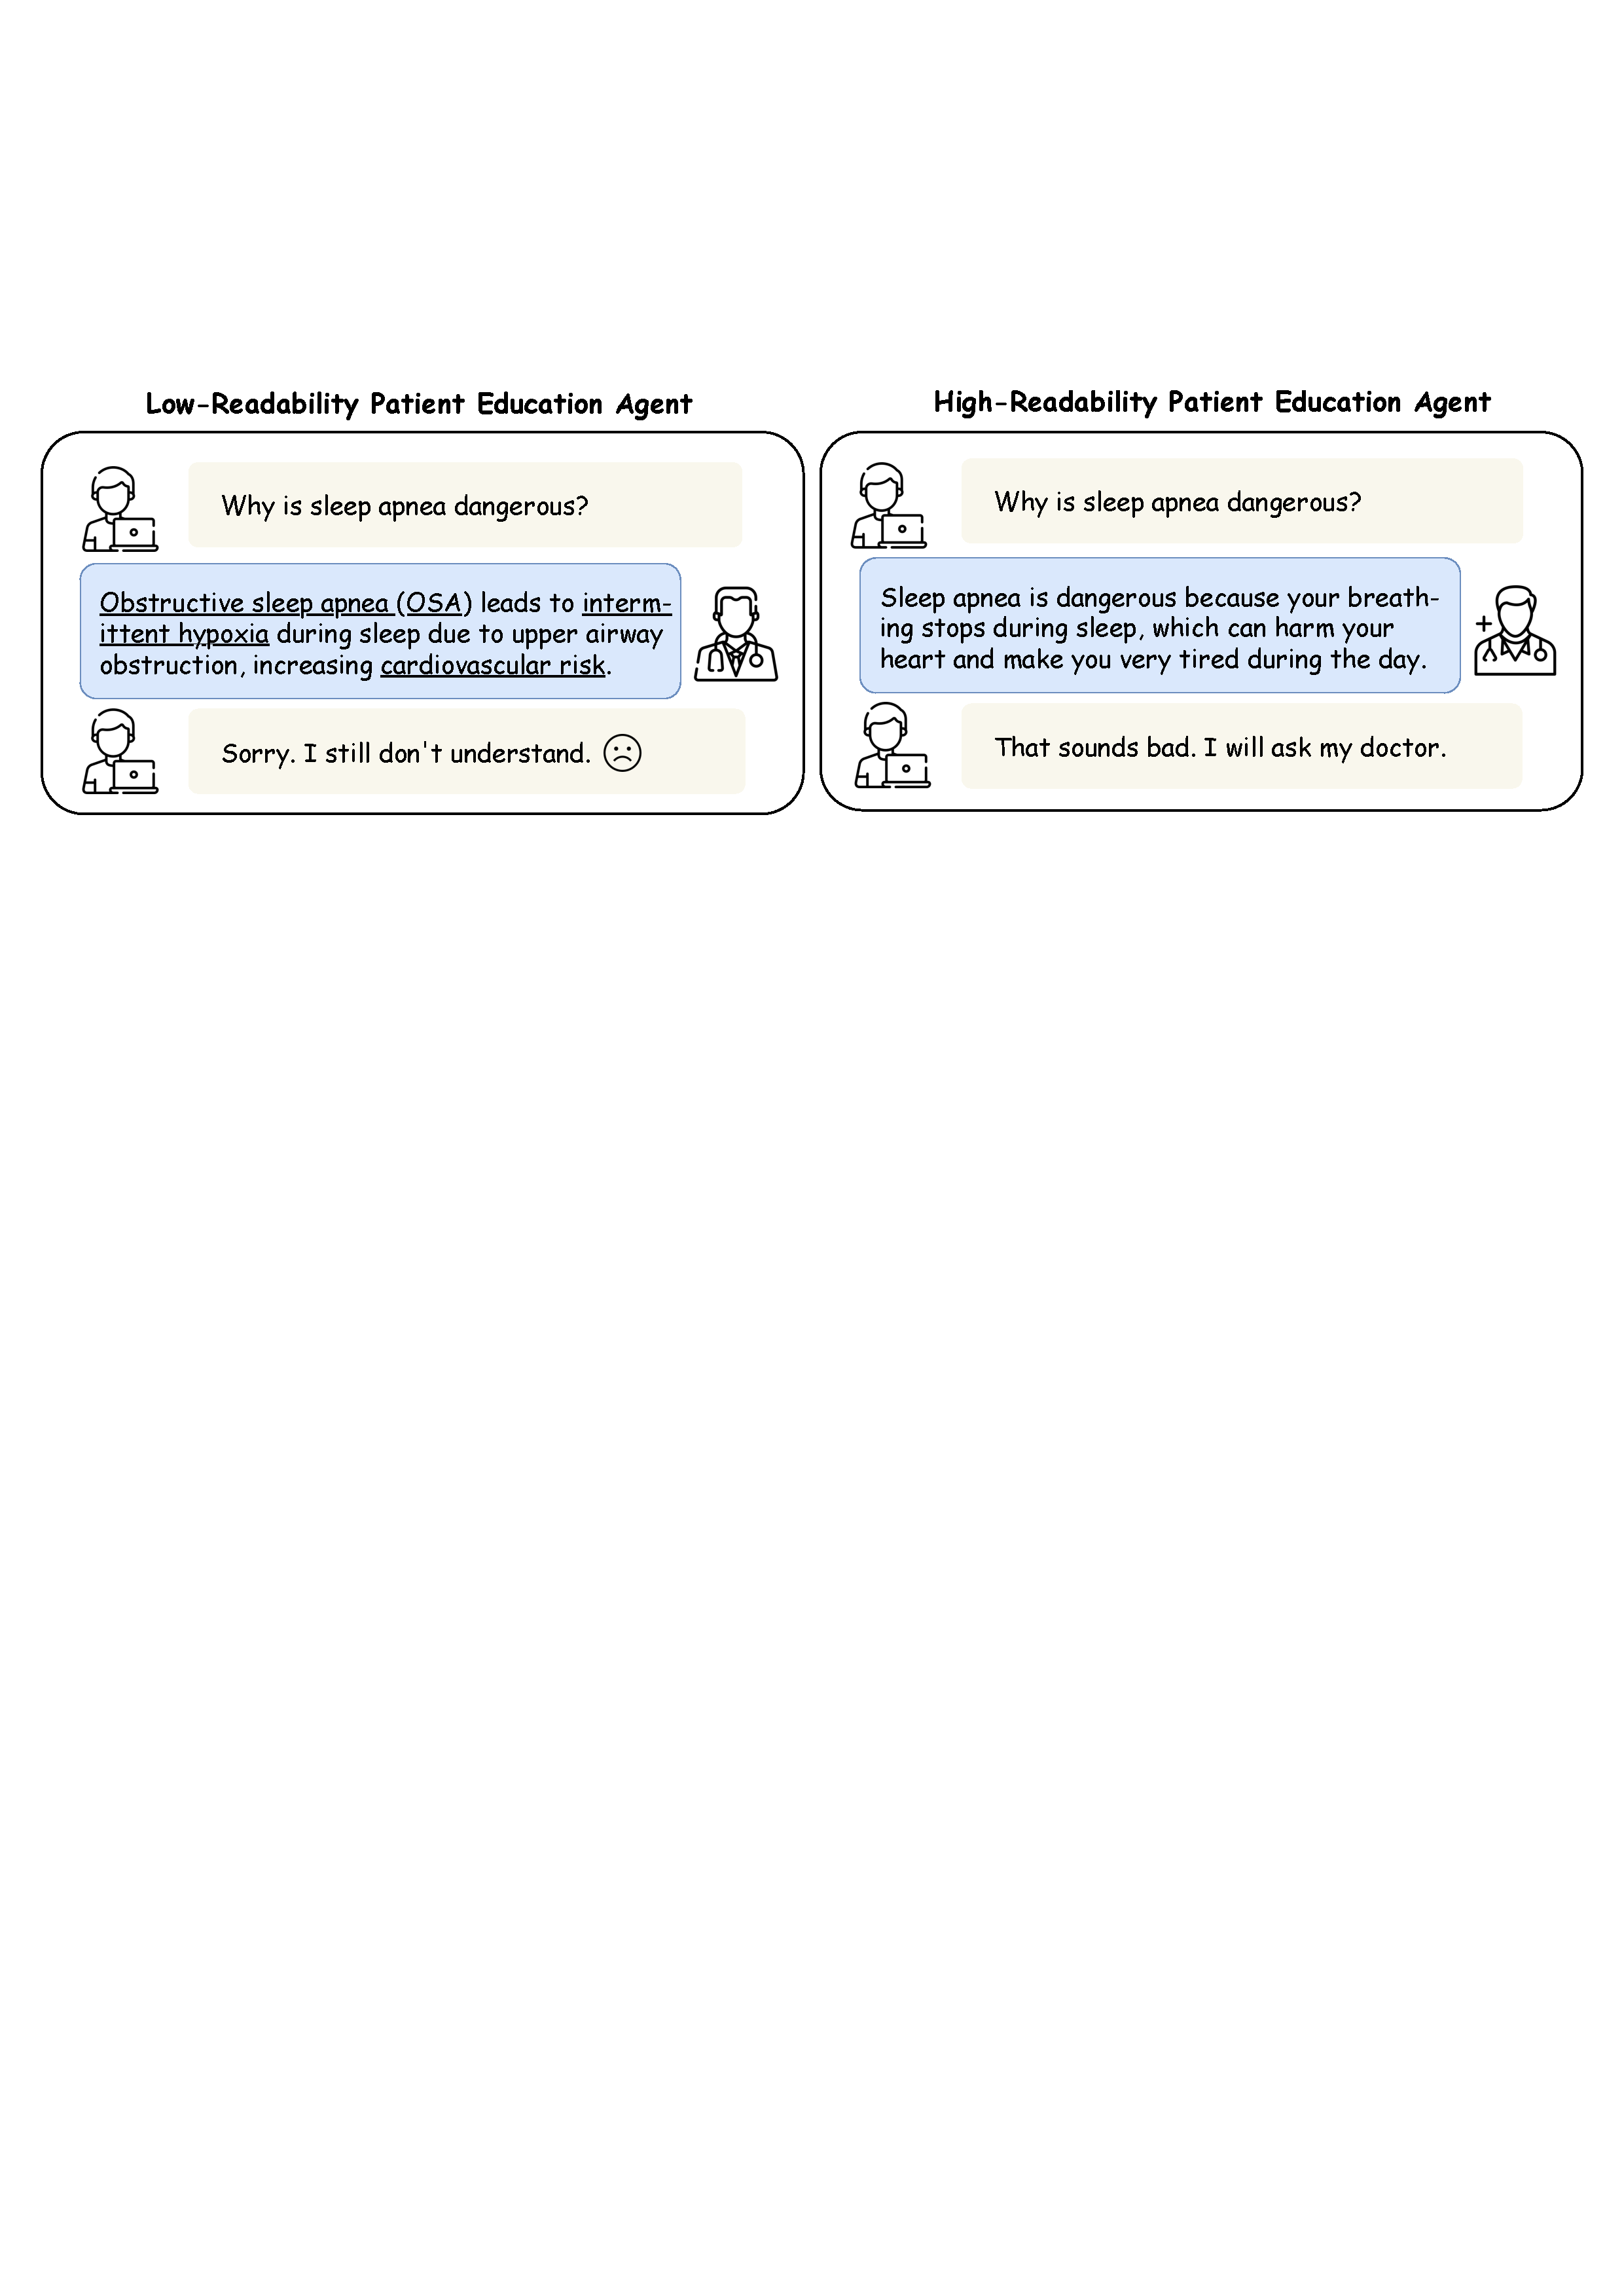
\includegraphics[width=1.0\textwidth]{figs/teaser_figv2.pdf}
    \caption{
        Two examples of user interactions with low- and high-readability public health agents. Medical jargon is underscored for the low-readability agent.
    }
    \label{fig:repqa-teaser}
\end{figure}

As shown in Figure~\ref{fig:repqa-teaser}, users without a medical professional background may find low-readability responses filled with medical jargon difficult to comprehend, whereas a plain-language answer can convey the same essential information more accessibly.
Moreover, state-of-the-art LLMs are increasingly optimized for complex reasoning~\citep{shao2024deepseekmath},
raising the question of whether these gains come at the expense of readability.
More advanced reasoning may lead to more technical responses that are harder for lay users to understand.

To evaluate the capabilities of LLMs in solving healthcare and medical problems, multiple benchmarks have been curated from diverse sources and presented in various formats~\citep{singhal2023large, lievin2024can, thirunavukarasu2023large}.
For instance, MedQA~\citep{jin2021disease}, MedMCQA~\citep{pal2022medmcqa}, MMLU~\citep{hendrycks2020measuring, wang2024mmlu}, and PubMedQA~\citep{jin2019pubmedqa} contain multiple-choice questions sourced from medical licensing examinations or PubMed articles, while LiveQA~\citep{abacha2017overview} and MedicationQA~\citep{abacha2019bridging} focus on long-form question answering for medicine-related problems.
Recent efforts have shifted toward more complex clinical tasks requiring multi-step reasoning and decision-making~\citep{yao2024medqa, chen2025benchmarking,nori2024medprompt,saab2024capabilities}, as well as incorporating additional modalities such as electronic health records~\citep{ou2025experience, bardhan2022drugehrqa, kweon2024ehrnoteqa}, radiology~\citep{zuo2025medxpertqa, liu2021slake}, and pathology~\citep{he2020pathvqa,lu2024multimodal}.
However, these benchmarks mainly evaluate the factual or reasoning accuracy of LLMs against professional examinations or specialized clinical tasks, rather than the readability of responses delivered to lay users.
% As summarized in Table~\ref{tab:dataset_comparison}, \repqa is the first to comprehensively evaluate the readability of LLM-generated responses to healthcare-related questions, using a dataset composed of publicly available medical queries from lay users.

\begin{table*}[t]
    \centering
    \caption{The comparison between \repqa and the existing healthcare benchmark datasets.}
    \resizebox{\textwidth}{!}{
    \begin{tabular}{ccccc}
    \toprule
    Dataset & Answer Format & Sources of Questions & Evaluation Metrics & Target Audience \\
    \midrule
    \midrule
    MedQA~\citep{jin2021disease} & Multiple Choice & Medical Examination & Accuracy & Medical Professionals \\
    MedMCQA~\citep{pal2022medmcqa} & Multiple Choice & Medical Examination & Accuracy & Medical Professionals \\
    MMLU~\citep{hendrycks2020measuring} & Multiple Choice & Medical Examination & Accuracy & Academic \\
    PubMedQA~\citep{jin2019pubmedqa} & Multiple Choice & PubMed Abstract & Accuracy & Clinical Researchers \\
    LiveQA~\citep{abacha2017overview} & Long Answer & National Library of Medicine & Human Evaluation & Consumers \\
    MedicationQA~\citep{abacha2019bridging} & Long Answer & MedlinePlus \& DailyMed & Human Evaluation & Medicine Consumers \\
    JAMA \& Medbullets~\citep{chen2025benchmarking} & Long Answer \& Multiple Choice & JAMA Challenge \& USMLE & NLG Metrics \& Accuracy & Medical Professionals \\
    \midrule
    \repqa & Long Answer & Public Health FAQs \& Experts & Readability \& Informativeness & Lay Users / Patients \\
    \bottomrule
    \end{tabular}
    }
    \label{tab:dataset_comparison}
\end{table*}

Beyond evaluation, a related line of research studies how to \emph{control} the complexity or reading level of text generated by LLMs.
Three main strategies have been explored:
(1) prompt- or instruction-based methods that modulate output difficulty by varying instructions or providing exemplars~\citep{tran2024readctrl, malik2024tarzan, barayan2024analysing, pu2023chatgpt};
(2) fine-tuning-based methods, e.g., \citet{chi2023learning} fine-tune language models on same-level paraphrasing datasets, and \citet{ribeiro-etal-2023-generating} employ PPO~\citep{schulman2017proximal} with the measured reading level~\citep{kincaid1975derivation} as a reward signal;
and (3) decoding-based methods that incorporate constraints during text generation~\citep{ribeiro-etal-2023-generating,luo2022readability}.
Several studies have further investigated the readability of LLM-generated responses regarding certain cancers~\citep{hershenhouse2024accuracy,gencer2024readability} or patient education handouts~\citep{swisher2024enhancing}.
While most prior work focuses on text summarization, \repqa specifically targets the readability of LLMs in patient education QA tasks.

In this study, a multidisciplinary team comprised of computer science, nursing, and public health experts introduced \textbf{\repqa} to conduct a comprehensive investigation into the \textbf{RE}adability of LLMs in \textbf{P}atient \textbf{E}ducation question-\textbf{A}nswering (QA) tasks.
A key strength of \repqa lies in its expert-grounded foundation: it comprises a high-quality test set with 533 QA pairs curated from 27 online public health resources.
% , all reviewed by professionals in nursing, public health, and clinical communication.
Different from prior related benchmarks (Table~\ref{tab:dataset_comparison}), \repqa focuses on frequently asked health questions from lay users or patients, and evaluates the readability of generated responses, an axis that prior healthcare benchmarks largely overlook, rather than only the underlying factual knowledge of the LLMs.
Additionally, we collected a large-scale corpus of 36,060 public health questions to serve as a post-training dataset, supporting the exploration of readability-enhancement strategies.

We evaluated 19 LLMs on \repqa using three readability metrics (Flesch-Kincaid grade level~\citep{kincaid1975derivation}, professional-language proportion, and Yngve depth~\citep{yngve1960model}) and an informativeness metric (the informative cosine between a response and its reference answer).
Our study targeted three capabilities: (i) answering at a specified reading level, (ii) inferring the appropriate level for a question, and (iii) using readability as a reward signal.
We found that current models mostly missed target levels and poorly identified appropriate levels, limiting their applicability for public-health agents.
We then benchmarked five existing readability-improvement strategies, including training-free controls (instruction-based prompting~\citep{ribeiro-etal-2023-generating,malik2024tarzan}, CoT~\citep{wei2022chain}, and lookahead decoding~\citep{ribeiro-etal-2023-generating}) and reinforcement-learning fine-tuning (GRPO~\citep{shao2024deepseekmath} and DAPO~\citep{yu2025dapo}).
Readability-aware post-training yielded large gains in readability metrics but could reduce the informativeness of responses due to over-simplification, underscoring a difficult readability–informativeness trade-off.
This study will offer insights for future work on developing trustworthy healthcare agents and educational domains~\citep{wang2024large}.
In summary, our contributions are listed as follows:
\begin{itemize}[leftmargin=*]
\item We introduced \repqa, an expert-crafted benchmark for patient education QA aimed at lay users, with three readability metrics (Flesch–Kincaid grade, professional-language proportion, and Yngve depth), an informativeness metric (the informative cosine between a response and its reference answer), and a large-scale (36,060) expert-reviewed public health questions for post-training.

\item We conducted a study on 19 LLMs, revealing that most models failed to (i) generate at requested reading levels and (ii) identify an appropriate level for a given question.

\item We benchmarked a range of existing strategies for improving LLM readability, spanning training-free control (prompting, chain-of-thought, and lookahead decoding) and reinforcement-learning fine-tuning (GRPO and DAPO). Readability improved substantially, but often at the expense of informativeness, highlighting a challenging readability–informativeness trade-off.
\end{itemize}

\section{Results}\label{sec:results}

\subsection{Overview of \repqa}

\repqa is a benchmark for systematically evaluating the readability of LLMs in patient education question answering.
It comprises a high-quality collection of patient education QA pairs, each with an expert-grounded reference answer, together with a large-scale set of unlabeled questions for training.
\begin{figure}[htbp]
    \centering
    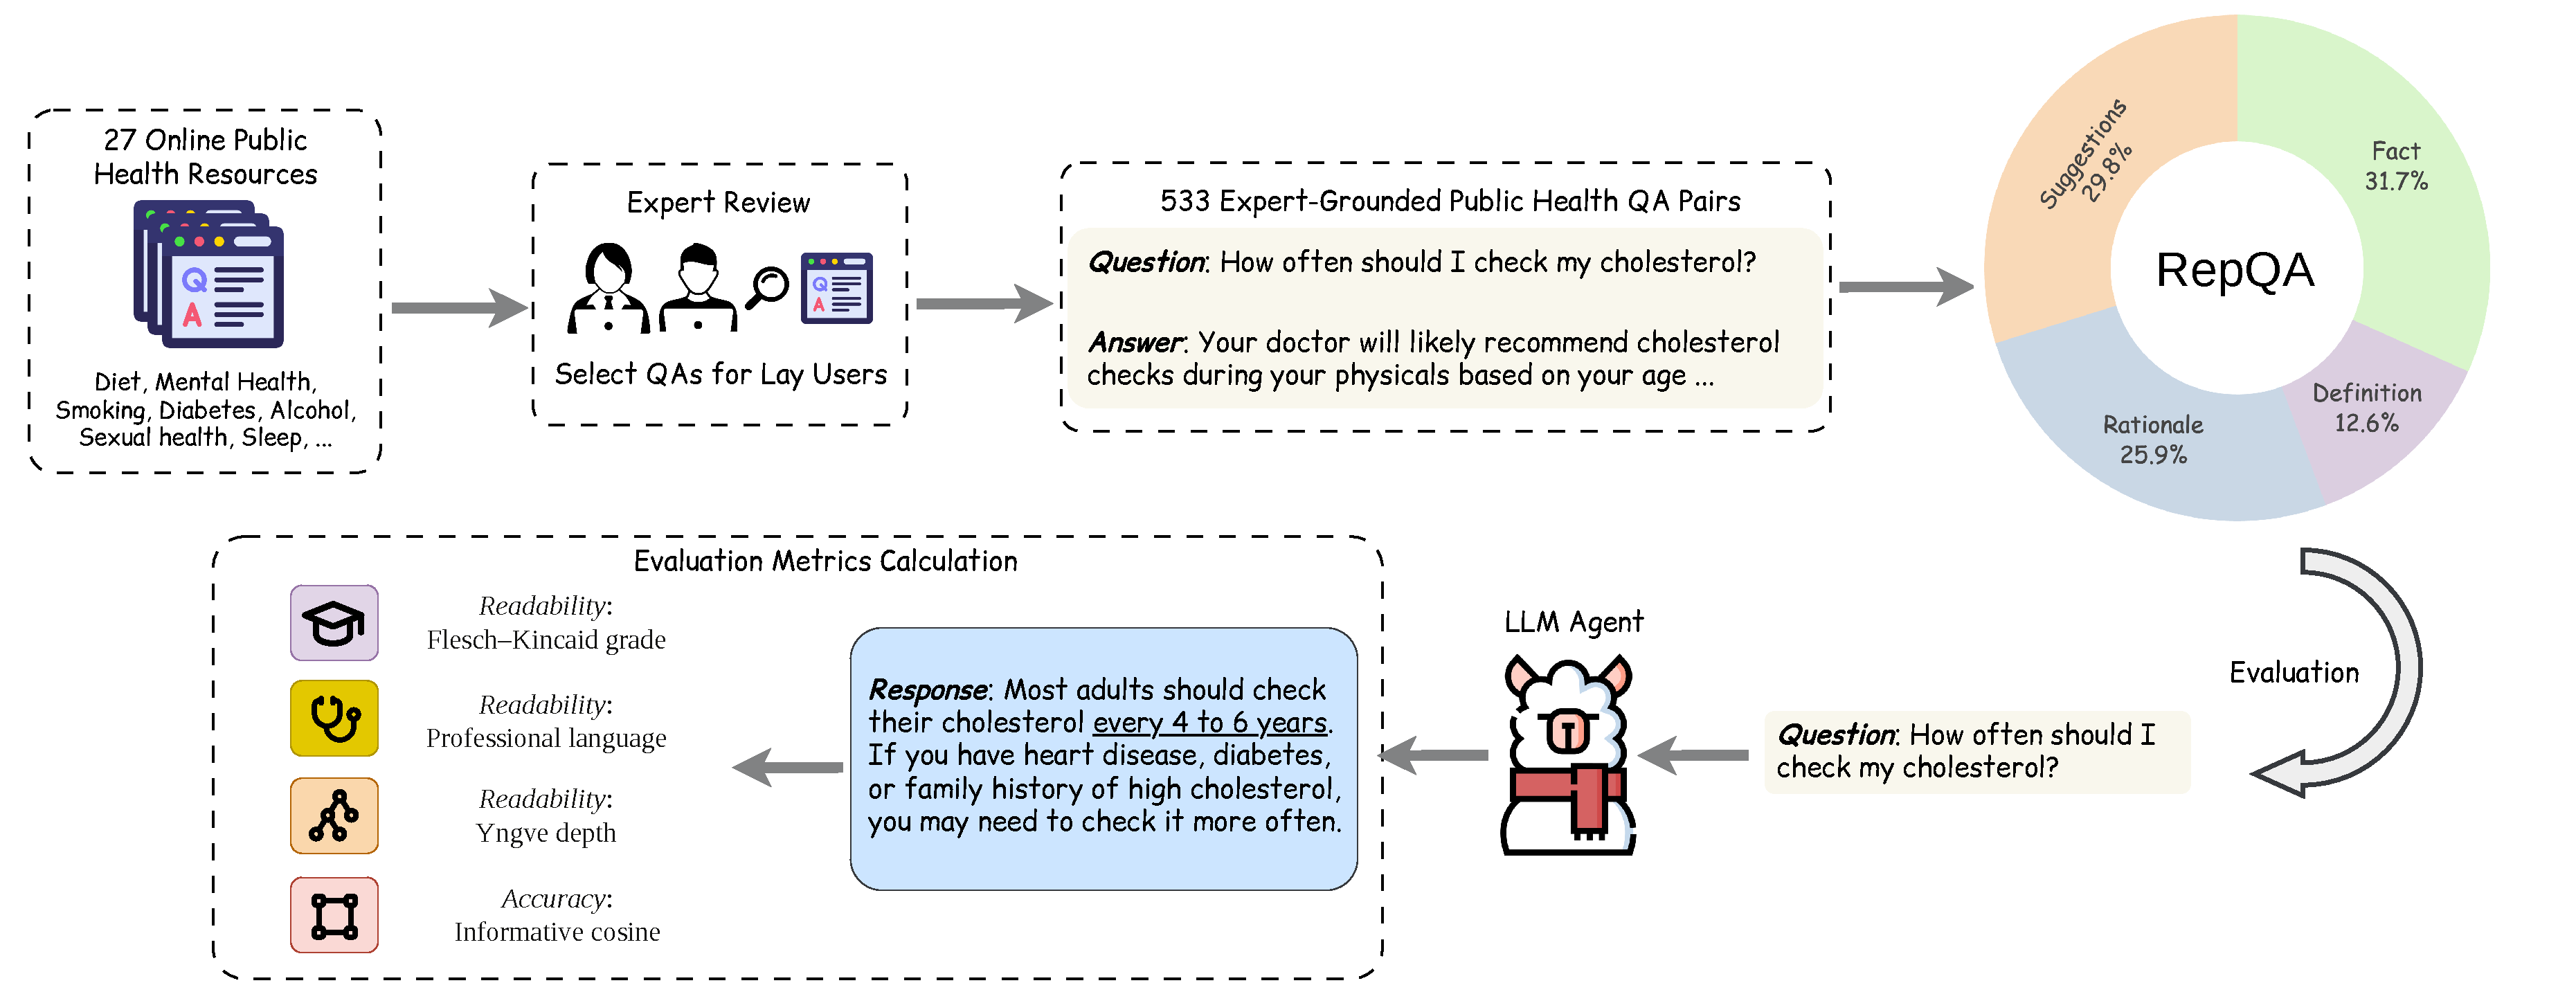
\includegraphics[width=1.0\textwidth]{figs/workflow_new.pdf}
    \caption{
        Overview of the \repqa benchmark. \textbf{Top:} dataset construction --- patient-education QA pairs are collected from 27 online public health resources and filtered by domain experts to suit lay users, yielding 533 expert-grounded QA pairs (each with an auto-generated multiple-choice counterpart) that span four categories (Suggestion, Fact, Definition, and Rationale). \textbf{Bottom:} evaluation --- given a question, an LLM agent generates a free-form response, which is scored by three readability metrics (Flesch--Kincaid grade, professional language, and Yngve depth) and an informativeness metric (the informative cosine between the response and the expert reference answer).
    }
    \label{fig:workflow}
\end{figure}

Figure~\ref{fig:workflow} illustrates the overall dataset construction and evaluation pipeline: the dataset is curated through expert review, while the evaluation involves both readability assessment and an informativeness measure against the reference answers.
The construction procedure, evaluation metrics, and study design are detailed in the Methods (Section~\ref{sec:methods}).

\begin{table*}[t]
    \centering
    \caption{Examples and distribution of question categories in \repqa. Each question is accompanied by a corresponding reference answer.}
    \resizebox{\textwidth}{!}{
    \begin{tabular}{cp{15cm}c}
    \toprule
    Category & Example \& Reference Answer & Proportion \\
    \midrule
    \midrule
    \multirow{4}{*}{Suggestion} & \textbf{Q:} How can I quit smoking? & \multirow{4}{*}{29.8\%} \\
    & \textbf{A:} Commit to a quit day, choose a method for quitting (cold turkey or weaning down), talk to your doctor about medications to help quit, make a plan for when you quit on how to resist temptations, remove triggers, and have replacement activities, and then quit on your quit day! & \\
    \midrule
    \multirow{3}{*}{Fact} & \textbf{Q:} What are the chemicals in cigarettes? &  \multirow{3}{*}{31.7\%} \\
    & \textbf{A:}There are over 7,000 chemicals in cigarettes including arsenic, formaldehyde, tar, nicotine, and carbon monoxide, all of which are dangerous to your health. & \\
    \midrule
    \multirow{4}{*}{Definition} & \textbf{Q:} What is the Mediterranean Diet? & \multirow{4}{*}{12.6\%} \\
    & \textbf{A:} A Mediterranean diet is considered a healthy option as it emphasizes fruits and vegetables, whole grains, beans and legumes, low-fat dairy products, fish and poultry, and vegetable oils. It also limits sugars, processed foods, and fatty meats. & \\
    \midrule
    \multirow{3}{*}{Rationale} & \textbf{Q:} Why is blood pressure called a "silent killer"? & \multirow{3}{*}{25.9\%} \\
    & \textbf{A:} High blood pressure is sometimes called a silent killer because it can have no physical symptoms; however, the high blood pressure can damage arteries risking serious health events like heart attack or stroke. & \\
    \bottomrule
    \end{tabular}
    }
    \label{tab:dataset_category}
\end{table*}

The evaluation set of \repqa contains 533 QA pairs curated from 27 authoritative online public health resources and reviewed by domain experts in nursing, public health, and clinical communication.
Each question is phrased in plain language, without user profiles, and is accompanied by a reference answer.
As shown in Table~\ref{tab:dataset_category}, the QA pairs span four categories that capture common types of public health inquiries from lay users: \textit{Suggestion} (questions seeking advice), \textit{Fact} (questions requesting objective, verifiable information), \textit{Definition} (questions asking for explanations of medical terms or conditions), and \textit{Rationale} (questions seeking justifications behind medical guidance).
To enable informativeness assessment of free-form responses, each QA pair includes an expert-grounded reference answer, against which a generated response is compared via the informative cosine (IC).
In addition, \repqa provides a large-scale collection of 36,060 expert-reviewed public health questions spanning topics such as sleep, exercise, smoking, weight, diet, HIV care, mental health, cardiovascular disease, diabetes, cholesterol, and SOGI, supporting the exploration of readability-enhancement strategies such as reinforcement learning with verifiable readability rewards.

Using \repqa, we studied three research questions concerning LLMs' ability to adapt, assess, and optimize readability:
(RQ1) can LLMs generate responses at a specified reading level?
(RQ2) can LLMs determine what readability is needed for a given question?
and (RQ3) can readability serve as a reward signal?
We evaluated 19 LLMs, including 5 proprietary models and 14 open-source models, alongside five readability-enhancement strategies. The full experimental setup, including the list of evaluated models and configurations, is provided in Section~\ref{sec:exp_setup}.

\subsection{LLMs struggle to generate responses at a specified reading level}

People with different educational backgrounds have varying health literacy, so a healthcare agent should be able to adapt the readability of its answers to a requested level (RQ1).
We set a target score, i.e., 6 for the Flesch–Kincaid (FK) grade level and 0 for the professional-language (PL) score, and prompted each model to answer the queries accordingly. $\pi{=}6$ approximates a 5th-grade level intended to be broadly accessible, and $\rho{=}0$ denotes the absence of medical jargon.
As shown in Table~\ref{tab:repqa-main}, most models struggled to hit the target, often overshooting complexity or, when simplifying, omitting qualifiers.
Across the four categories, \textit{definition} was the easiest, with the lowest readability scores.

\begin{table*}[t]
\centering
\caption{Benchmarking proprietary and open-source LLMs with the \repqa{} metric suite. PL = Professional Language ($\downarrow$ less jargon), FK = Flesch--Kincaid Grade (target $\approx 6$), YD = Yngve Depth ($\downarrow$ simpler syntax), IC = Informative Cosine ($\uparrow$ more informative).}
\label{tab:repqa-main}
\small
\setlength{\tabcolsep}{3pt}
\resizebox{\linewidth}{!}{
\begin{tabular}{l cccc cccc cccc cccc}
\toprule
 & \multicolumn{4}{c}{Suggestion} & \multicolumn{4}{c}{Fact} & \multicolumn{4}{c}{Rationale} & \multicolumn{4}{c}{Definition} \\
\cmidrule(lr){2-5} \cmidrule(lr){6-9} \cmidrule(lr){10-13} \cmidrule(lr){14-17}
Model & PL$\downarrow$ & \textbf{FK$\rightarrow6$} & YD$\downarrow$ & IC$\uparrow$ & PL$\downarrow$ & \textbf{FK$\rightarrow6$} & YD$\downarrow$ & IC$\uparrow$ & PL$\downarrow$ & \textbf{FK$\rightarrow6$} & YD$\downarrow$ & IC$\uparrow$ & PL$\downarrow$ & \textbf{FK$\rightarrow6$} & YD$\downarrow$ & IC$\uparrow$ \\
\midrule
\multicolumn{17}{c}{\textbf{Proprietary Models (latest)}} \\
\midrule
GPT-5.5 & 2.55 & 11.08 & \underline{0.19} & 0.67 & 3.44 & 14.19 & \underline{1.11} & 0.74 & \underline{5.51} & 12.00 & 0.29 & \underline{0.75} & \underline{5.40} & 11.78 & \textbf{0.07} & 0.77 \\
GPT-5.4 & 2.08 & 15.90 & 1.67 & 0.67 & \textbf{2.65} & 15.00 & 1.29 & 0.74 & \textbf{4.33} & 13.68 & \underline{0.26} & 0.74 & \textbf{5.24} & 13.53 & 0.76 & 0.77 \\
GPT-5.1 & 2.24 & \textbf{8.24} & \textbf{0.04} & 0.65 & \underline{3.02} & \textbf{11.11} & \textbf{0.54} & 0.74 & 5.85 & \textbf{9.01} & \textbf{0.00} & 0.74 & 6.05 & \underline{10.90} & \underline{0.19} & 0.78 \\
GPT-4.1 & \textbf{1.62} & \underline{8.30} & 1.36 & \underline{0.71} & 3.12 & \underline{11.37} & 3.22 & \textbf{0.78} & 6.36 & \underline{9.84} & 2.42 & \textbf{0.77} & 7.50 & 10.95 & 2.58 & \underline{0.81} \\
GPT-4.1-mini & \underline{2.02} & 9.15 & 1.93 & \textbf{0.72} & 4.14 & 11.49 & 3.22 & \underline{0.77} & 7.01 & 10.70 & 3.06 & \textbf{0.77} & 8.56 & \textbf{10.71} & 2.92 & \textbf{0.82} \\
\midrule
\multicolumn{17}{c}{\textbf{Open-Source Models}} \\
\midrule
LLaMA3.1-8B & 2.08 & 8.15 & 0.28 & 0.68 & 3.89 & 9.21 & 0.62 & 0.75 & 7.12 & 9.39 & 0.50 & 0.74 & 7.87 & 10.44 & 1.01 & 0.79 \\
Qwen2.5-7B & 1.75 & \textbf{7.72} & 1.21 & 0.69 & 3.64 & 9.99 & 2.83 & \textbf{0.77} & 6.33 & 9.79 & 2.70 & \textbf{0.76} & 7.54 & 10.26 & 3.04 & \underline{0.81} \\
BioMistral-7B & 2.88 & 8.70 & 3.05 & 0.67 & 4.08 & 9.50 & 3.50 & 0.73 & 7.97 & \underline{9.37} & 2.98 & 0.72 & 8.05 & 10.38 & 3.08 & 0.78 \\
Phi-4 & 1.56 & 8.03 & 0.28 & 0.69 & 3.58 & 9.54 & 1.05 & \underline{0.76} & 6.72 & 10.07 & 0.95 & \underline{0.75} & 7.09 & 11.00 & 1.78 & 0.80 \\
Yi-1.5-9B & 1.83 & 9.17 & 1.52 & 0.69 & 4.52 & 10.21 & 2.64 & \underline{0.76} & 6.72 & 10.57 & 2.52 & 0.74 & 8.52 & 11.50 & 2.75 & 0.80 \\
Mistral-7B & 1.97 & 8.10 & 1.22 & 0.68 & 3.76 & 9.27 & 2.25 & \underline{0.76} & 7.10 & 10.52 & 2.58 & \underline{0.75} & 8.18 & 10.81 & 2.82 & 0.80 \\
InternLM3-8B & \underline{1.53} & 8.38 & \textbf{0.04} & 0.67 & 2.98 & 9.52 & \underline{0.22} & 0.73 & 5.38 & 10.13 & \underline{0.10} & 0.73 & \textbf{4.65} & 11.04 & \underline{0.77} & 0.77 \\
Gemma-3-12B & 1.59 & 7.97 & 0.29 & 0.66 & \underline{2.09} & \textbf{8.60} & 1.14 & 0.74 & \underline{5.33} & \textbf{8.78} & 1.02 & 0.73 & \underline{4.92} & \textbf{8.77} & 1.10 & 0.79 \\
Qwen2.5-14B & 2.03 & 8.33 & 1.36 & \underline{0.70} & 3.42 & 9.61 & 2.38 & \textbf{0.77} & 6.26 & 10.20 & 2.68 & \textbf{0.76} & 6.89 & 11.05 & 3.21 & \underline{0.81} \\
Qwen2.5-32B & \textbf{1.34} & \underline{7.90} & 1.18 & \textbf{0.71} & 3.45 & 9.66 & 2.47 & \textbf{0.77} & 5.80 & 10.39 & 2.77 & \textbf{0.76} & 6.71 & 10.48 & 2.94 & \underline{0.81} \\
% \multicolumn{17}{c}{\textbf{Newly Added Open-Source Models}} \\
% \midrule
Qwen3-8B & 2.11 & 8.45 & 1.65 & \underline{0.70} & 3.39 & 10.76 & 3.06 & \textbf{0.77} & 7.55 & 10.32 & 2.41 & \textbf{0.76} & 7.16 & 10.73 & 2.61 & \textbf{0.82} \\
Qwen3-14B & 1.78 & 7.93 & 1.04 & \underline{0.70} & 3.30 & 10.79 & 2.39 & \textbf{0.77} & 6.47 & 10.64 & 2.16 & \textbf{0.76} & 8.66 & 10.69 & 2.13 & \underline{0.81} \\
Qwen3-32B & 2.08 & 8.08 & 0.76 & \underline{0.70} & 3.31 & 10.32 & 1.69 & \textbf{0.77} & 6.18 & 10.55 & 1.51 & \textbf{0.76} & 8.17 & 11.06 & 2.00 & 0.80 \\
Gemma-3-27B & 1.58 & 8.28 & \underline{0.11} & 0.66 & \textbf{1.77} & \underline{9.12} & \textbf{0.14} & 0.74 & \textbf{4.15} & 9.38 & \textbf{0.00} & 0.71 & 5.04 & \underline{9.12} & \textbf{0.00} & 0.78 \\
\bottomrule
\end{tabular}
}
\end{table*}

To further probe readability control, we evaluated a set of representative models, spanning non-thinking models (LLaMA~3.1-8B, Qwen-3-30B) and thinking models (DeepSeek-R1-Distill-Qwen, Qwen-3-30B-Thinking, GPT-4.1), focusing on their ability to match requested reading levels.
We set four target levels, i.e., 5th grade, middle school, high school, and college, corresponding to FK grade levels of 6, 9, 12, and 15.
\begin{figure}[htbp]
    \centering
    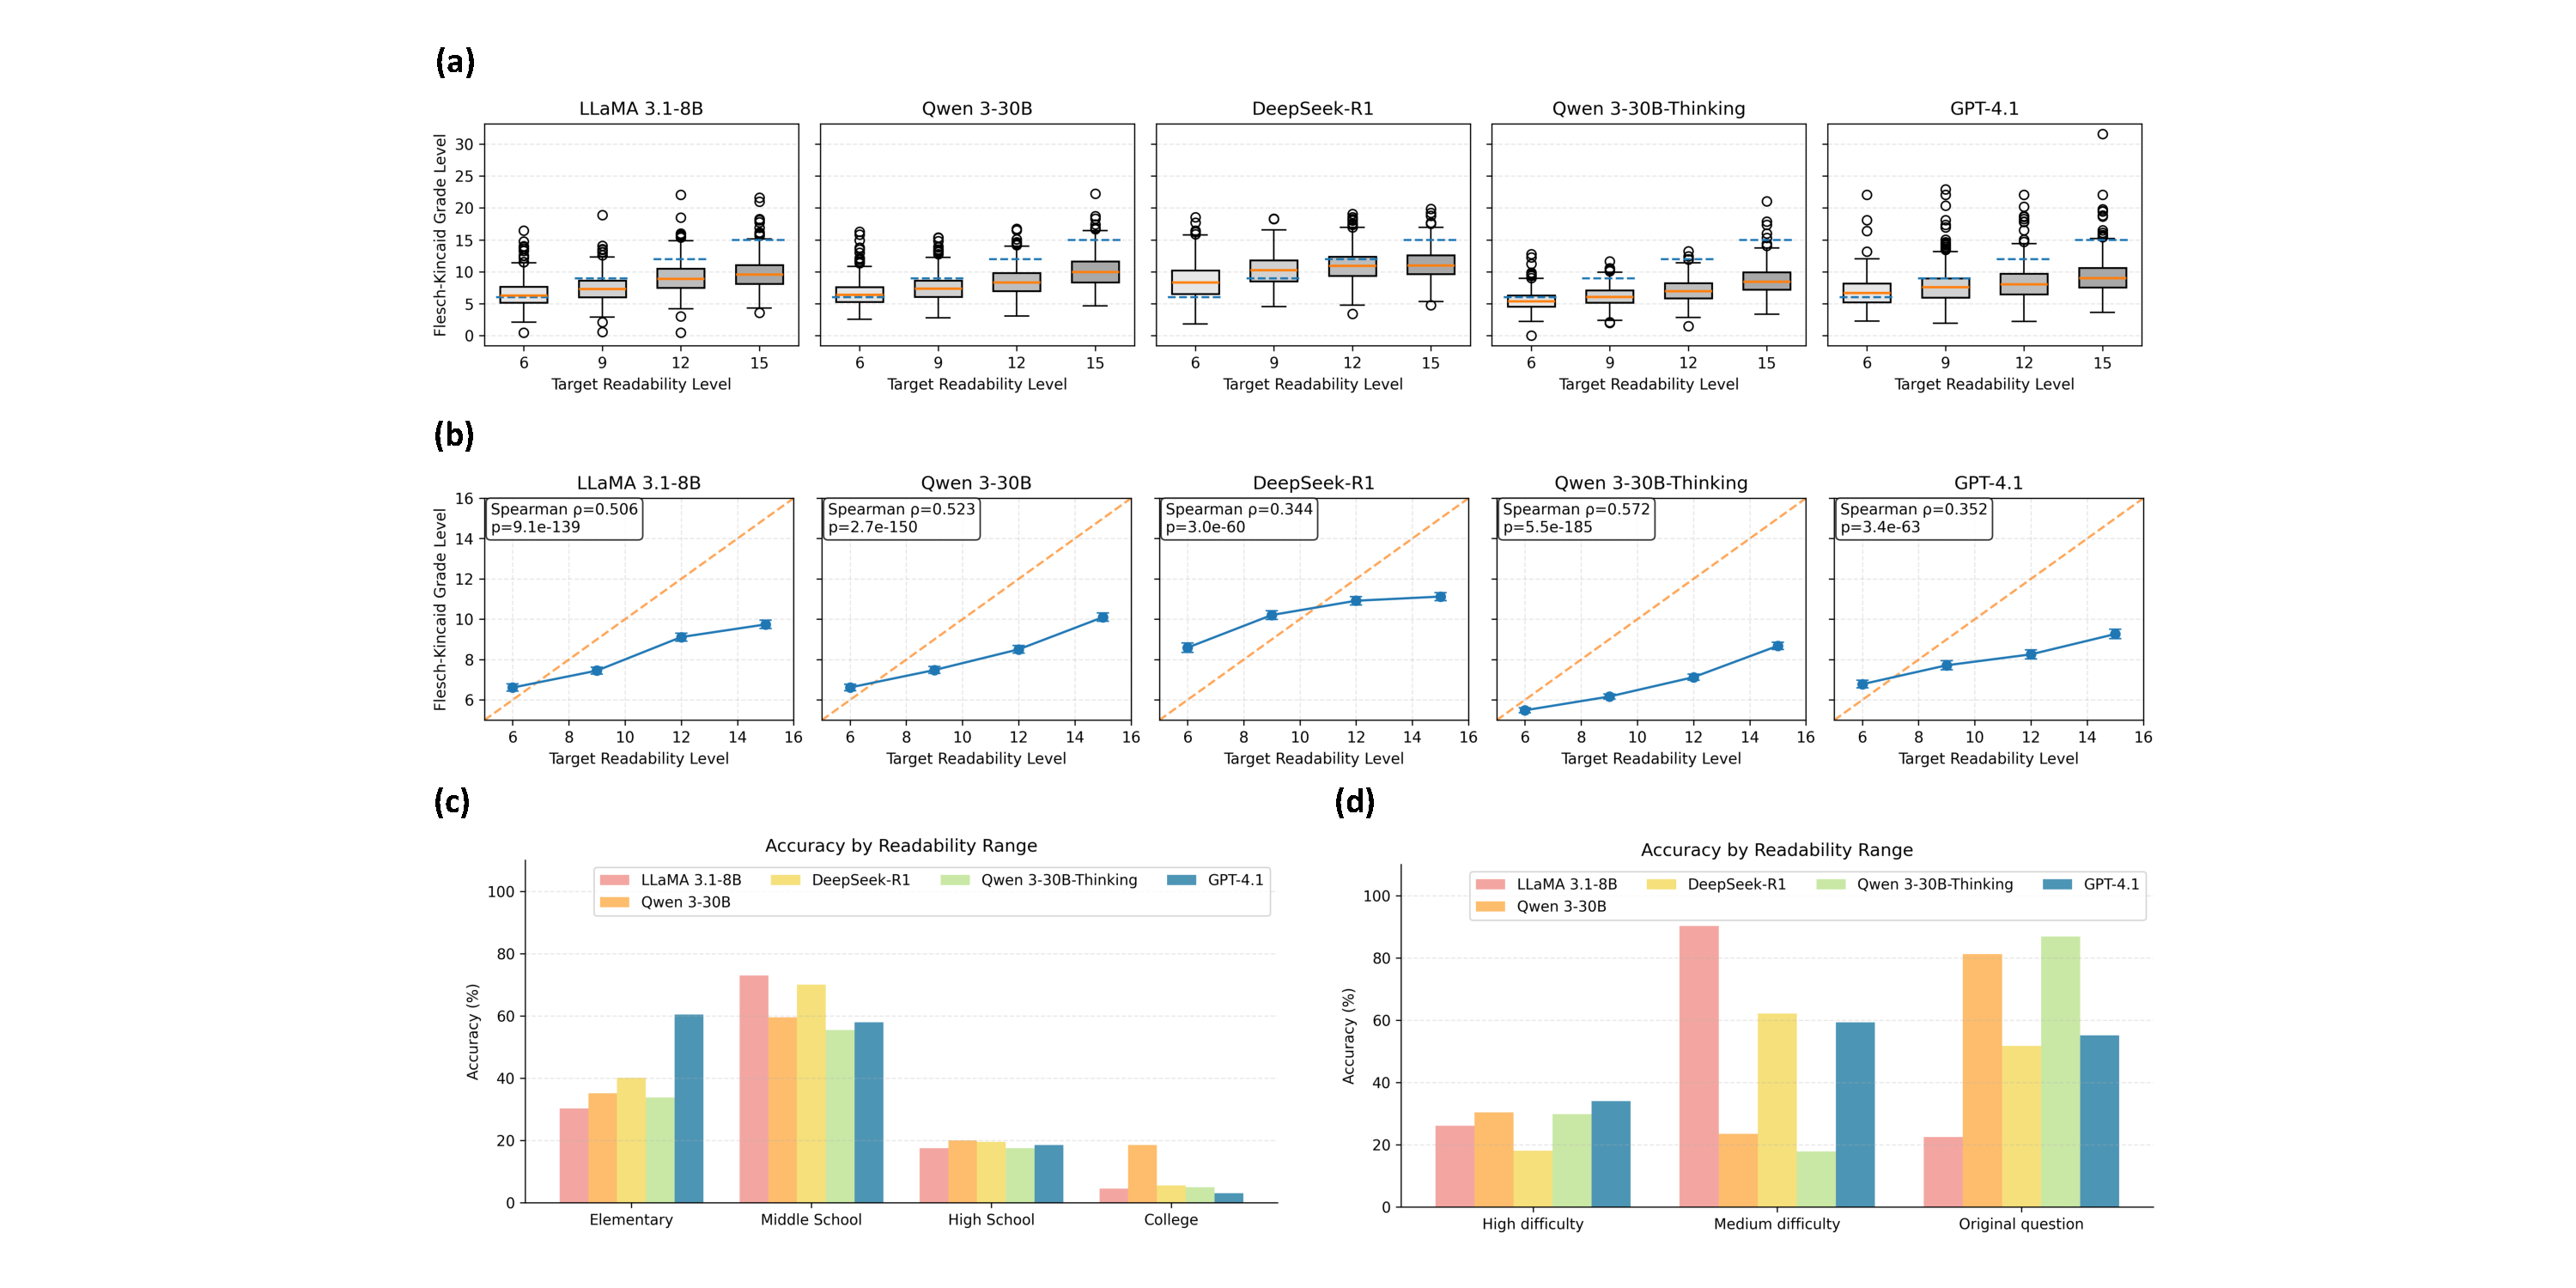
\includegraphics[width=1.0\linewidth]{figs/readability_study_new.pdf}
    \caption{
    Readability control and understanding across five models.
    \textbf{(a)} Achieved Flesch–Kincaid grades when instructed to write at target levels 6/9/12/15 (boxplots). Red horizontal lines mark the targets, and blue dashed lines mark the per-target mean grade.
    \textbf{(b)} Mean Flesch–Kincaid grade vs.\ target (error bars show 95\% CI).
    \textbf{(c)} Accuracy of classifying generated responses into Flesch–Kincaid buckets (Elementary/Middle/High/College).
    \textbf{(d)} Accuracy when classifying Original/Medium/High counterparts of the same question.
    }
    \label{fig:analysis}
\end{figure}

As shown in Figure~\ref{fig:analysis}(a,b), all models generally followed the intended direction (Spearman $\rho\approx 0.34\sim0.57$) but remained poorly calibrated: their FK grades consistently fell short of the targets, with larger deviations at higher levels.
In short, while models adjusted readability \emph{relatively}, they failed in \emph{absolute} alignment.

\subsection{LLMs poorly identify the readability required for a question}

We next examined whether poor control stems from a weak understanding of readability (RQ2).
We first tested whether models can recognize the reading level of existing text: we sampled 200 generated responses per bin (Elementary, Middle School, High School, College; mapped from FK grade) and asked models to classify the bin.
As shown in Figure~\ref{fig:analysis}(c), accuracy peaked at Middle School, was moderate at Elementary, and collapsed at High School and College.
This systematic bias toward lower buckets mirrored the undershoot observed for readability control.

We then studied whether LLMs understand differences in the medical knowledge required by a question.
For each question in \repqa, we prompted GPT-4o to generate two counterparts that vary only in the required domain knowledge (Medium and High).
Each model then classified the resulting variant.
As shown in Figure~\ref{fig:analysis}(d), performance was uneven across systems, e.g., LLaMA~3.1-8B was relatively strong on Medium but weak on Original, whereas Qwen-3-30B-Thinking excelled on Original yet remained low on High.
Across models, detection of High difficulty was uniformly poor, indicating limited sensitivity to advanced domain knowledge and helping explain the tendency to default to overly simple outputs.

\subsection{Readability can serve as a reward signal, but at an accuracy cost}

Reinforcement learning has shown promise for steering LLMs toward preferred behaviors. We therefore studied whether readability can act as a useful reward signal (RQ3).
We optimized readability using the reward in Eq.~\ref{equ:reward} within two reinforcement-learning algorithms, GRPO~\citep{shao2024deepseekmath} and DAPO~\citep{yu2025dapo}, the latter improving upon GRPO with decoupled clipping and dynamic sampling (Methods, Section~\ref{sec:methods}).
As training-free baselines we included three readability-control methods from \citet{ribeiro-etal-2023-generating}: \emph{Prompt} (instruction-based control, prompting the base model for simple, plain-language answers), \emph{CoT} (chain-of-thought prompting), and \emph{Lookahead} (a decoding method that at each step estimates the readability of candidate continuations via a short greedy lookahead and biases generation toward the target grade level). All three were applied to the base model with no fine-tuning.
Results are reported in Table~\ref{tab:post}.

The training-free controls traded off differently across the readability axes.
\emph{Prompt} sharply lowered the word-level grade (FK) and jargon (PL), but raised syntactic complexity (YD) and eroded informativeness (IC); \emph{Lookahead} pulled FK toward the target while best preserving IC among the non-RL methods, yet left jargon and syntax largely unchanged because its guidance optimizes FK alone; and \emph{CoT} produced less readable text with no meaningful gain in informativeness.
In contrast, RL fine-tuning (GRPO/DAPO) was the only approach that improved all four axes at once -- lowering FK, PL, and YD while retaining the highest IC -- since its reward jointly targets word choice, syntax, and faithfulness.
Both GRPO and DAPO improved readability; among them, DAPO yielded the largest gains, reducing the grade level by 41.4\% on average and the professional-language score by 73.3\%.
Moreover, DAPO outperformed vanilla GRPO on professional-language readability (53.4\% average reduction) while maintaining a comparable grade level (3.0\% difference).
Although RL fine-tuning largely retained informativeness (IC) at the aggregate level, the drive toward simpler text can still cost content fidelity: as the case study (Section~\ref{sec:case_study}) and the expert evaluation below show, the simplified responses sometimes omitted key facts, especially on \textit{Suggestion} and \textit{Fact}, highlighting the difficulty of simplifying without losing content.

\begin{table*}[t]
\centering
\caption{Readability-control strategies on the \repqa{} metric suite, per question type. For each base model we compared training-free controls -- \emph{Prompt} (instruction-based control), \emph{CoT} (chain-of-thought), and \emph{Lookahead} (readability-guided lookahead decoding, \citealp{ribeiro-etal-2023-generating}) -- against RL fine-tuning (\emph{DAPO}/\emph{GRPO}). PL = Professional Language ($\downarrow$), FK = Flesch--Kincaid Grade (target $\approx 6$), YD = Yngve Depth ($\downarrow$, raw), IC = Informative Cosine ($\uparrow$). Prompting and lookahead improve word-level readability (FK) but not syntactic complexity (YD); RL improves all axes while best retaining informativeness (IC). Within each base model, \textbf{bold} marks the best and \underline{underline} the second-best value per column.}
\label{tab:post}
\tiny
\setlength{\tabcolsep}{3pt}
\begin{tabular}{l cccc cccc cccc cccc}
\toprule
 & \multicolumn{4}{c}{Suggestion} & \multicolumn{4}{c}{Fact} & \multicolumn{4}{c}{Rationale} & \multicolumn{4}{c}{Definition} \\
\cmidrule(lr){2-5} \cmidrule(lr){6-9} \cmidrule(lr){10-13} \cmidrule(lr){14-17}
Model & PL$\downarrow$ & FK$\rightarrow6$ & YD$\downarrow$ & IC$\uparrow$ & PL$\downarrow$ & FK$\rightarrow6$ & YD$\downarrow$ & IC$\uparrow$ & PL$\downarrow$ & FK$\rightarrow6$ & YD$\downarrow$ & IC$\uparrow$ & PL$\downarrow$ & FK$\rightarrow6$ & YD$\downarrow$ & IC$\uparrow$ \\
\midrule
LLaMA3.1-8B & 2.08 & 8.15 & 0.28 & 0.68 & 3.89 & 9.21 & 0.62 & 0.75 & 7.12 & 9.39 & 0.50 & 0.74 & 7.87 & 10.44 & 1.01 & 0.79 \\
\scriptsize + Prompt & \underline{0.90} & 5.24 & 0.50 & 0.66 & 1.69 & 7.12 & 1.83 & 0.73 & 3.98 & 5.75 & 1.58 & 0.73 & 5.76 & \textbf{5.99} & 1.65 & 0.79 \\
\scriptsize + CoT & 3.08 & 10.25 & 4.11 & 0.61 & 2.22 & 9.89 & 3.90 & 0.70 & 5.22 & 9.65 & 3.28 & 0.70 & 8.85 & 9.65 & 3.07 & 0.76 \\
\scriptsize + Lookahead & 2.24 & 6.48 & 0.28 & 0.68 & 4.05 & 6.65 & 0.77 & 0.75 & 6.55 & 6.86 & 0.28 & 0.74 & 8.28 & 6.93 & 1.21 & 0.77 \\
\scriptsize + DAPO & \textbf{0.76} & \underline{5.83} & \textbf{0.02} & \textbf{0.72} & \textbf{0.57} & \underline{5.92} & \textbf{0.08} & \textbf{0.78} & \textbf{1.54} & \textbf{5.91} & \textbf{0.02} & \textbf{0.76} & \textbf{2.52} & \underline{6.20} & \textbf{0.12} & \underline{0.80} \\
\scriptsize + GRPO & 1.07 & \textbf{5.92} & \underline{0.13} & \underline{0.70} & \underline{1.64} & \textbf{5.92} & \underline{0.35} & \underline{0.76} & \underline{3.07} & \underline{5.88} & \underline{0.08} & \underline{0.75} & \underline{5.41} & 6.83 & \underline{0.46} & \textbf{0.81} \\
\midrule
Qwen3-8B & 2.11 & 8.45 & \underline{1.65} & \underline{0.70} & 3.39 & 10.76 & 3.06 & \underline{0.77} & 7.55 & 10.32 & \underline{2.41} & \underline{0.76} & 7.16 & 10.73 & 2.61 & \textbf{0.82} \\
\scriptsize + Prompt & \textbf{0.69} & 4.61 & 2.57 & 0.66 & \underline{1.33} & 5.10 & \underline{2.58} & 0.73 & \underline{3.17} & 5.33 & 2.52 & 0.72 & \textbf{3.86} & \textbf{5.14} & \underline{2.40} & 0.77 \\
\scriptsize + CoT & 1.67 & \underline{6.62} & 3.47 & 0.59 & 2.75 & \underline{6.82} & 3.07 & 0.74 & 6.39 & \textbf{6.44} & 2.62 & 0.71 & 5.26 & \underline{7.34} & 2.63 & 0.76 \\
\scriptsize + Lookahead & 2.00 & 6.73 & \textbf{1.04} & 0.70 & 3.54 & 7.57 & \textbf{2.09} & 0.76 & 5.90 & 7.92 & \textbf{2.29} & 0.75 & 6.55 & 8.25 & \textbf{2.38} & 0.80 \\
\scriptsize + DAPO & \underline{0.79} & \textbf{6.19} & 2.82 & 0.69 & \textbf{0.71} & \textbf{6.29} & 2.82 & 0.76 & \textbf{3.03} & \underline{6.45} & 2.67 & 0.73 & \underline{4.24} & 7.37 & 2.85 & 0.80 \\
\scriptsize + GRPO & 2.11 & 8.94 & 3.19 & \textbf{0.71} & 2.41 & 9.12 & 3.23 & \textbf{0.78} & 5.17 & 9.29 & 2.94 & \textbf{0.76} & 6.16 & 9.68 & 2.99 & \underline{0.81} \\
\midrule
Qwen3-4B & 1.80 & 7.97 & \underline{1.77} & 0.69 & 3.38 & 9.76 & 3.28 & \underline{0.77} & 7.90 & 9.75 & 2.55 & \textbf{0.76} & 6.56 & 9.87 & 2.65 & \underline{0.81} \\
\scriptsize + Prompt & 0.98 & 3.34 & 2.26 & 0.63 & \underline{1.32} & 4.62 & \underline{2.51} & 0.73 & \underline{3.55} & 4.39 & 2.40 & 0.71 & \underline{4.33} & \underline{4.39} & \textbf{2.36} & 0.76 \\
\scriptsize + CoT & \textbf{0.60} & \textbf{6.44} & 3.72 & 0.57 & 1.84 & \textbf{6.83} & 3.19 & 0.72 & 5.97 & \textbf{6.48} & 2.76 & 0.70 & 5.95 & \textbf{7.35} & 2.73 & 0.76 \\
\scriptsize + Lookahead & 1.93 & \underline{6.77} & \textbf{1.34} & \underline{0.70} & 3.32 & 7.58 & 2.83 & 0.76 & 5.78 & 7.81 & \textbf{2.19} & 0.75 & 6.13 & 7.82 & 2.61 & 0.79 \\
\scriptsize + DAPO & \underline{0.68} & 7.00 & 2.48 & 0.68 & \textbf{0.75} & \underline{7.14} & \textbf{2.47} & 0.76 & \textbf{2.19} & \underline{7.17} & \underline{2.36} & 0.73 & \textbf{3.43} & 7.75 & \underline{2.43} & 0.80 \\
\scriptsize + GRPO & 1.84 & 9.25 & 3.33 & \textbf{0.71} & 1.38 & 9.22 & 3.31 & \textbf{0.77} & 4.59 & 9.08 & 2.99 & \underline{0.75} & 5.74 & 9.72 & 2.96 & \textbf{0.81} \\
\bottomrule
\end{tabular}
\end{table*}

\paragraph{Expert evaluation}
We performed a manual inspection of the responses from Qwen2.5-7B and LLaMA3.1-8B, both post-trained via DAPO.
Specifically, we presented questions to 8 domain experts in a blind evaluation, in which experts were asked to select the superior response from a pair of randomized outputs.
Our results showed that in 75\% of the cases, experts favored the responses from LLaMA3.1-8B over those from Qwen2.5-7B.
This discrepancy with the metric-based ranking in Table~\ref{tab:post} suggested that static readability metrics may deviate from human perception.

\subsection{Case study: improved readability at the expense of informativeness}\label{sec:case_study}

\repqa revealed that, although GRPO/DAPO with a readability-based reward markedly improved readability, it can reduce the informativeness of responses.
\begin{figure}[htbp]
    \centering
    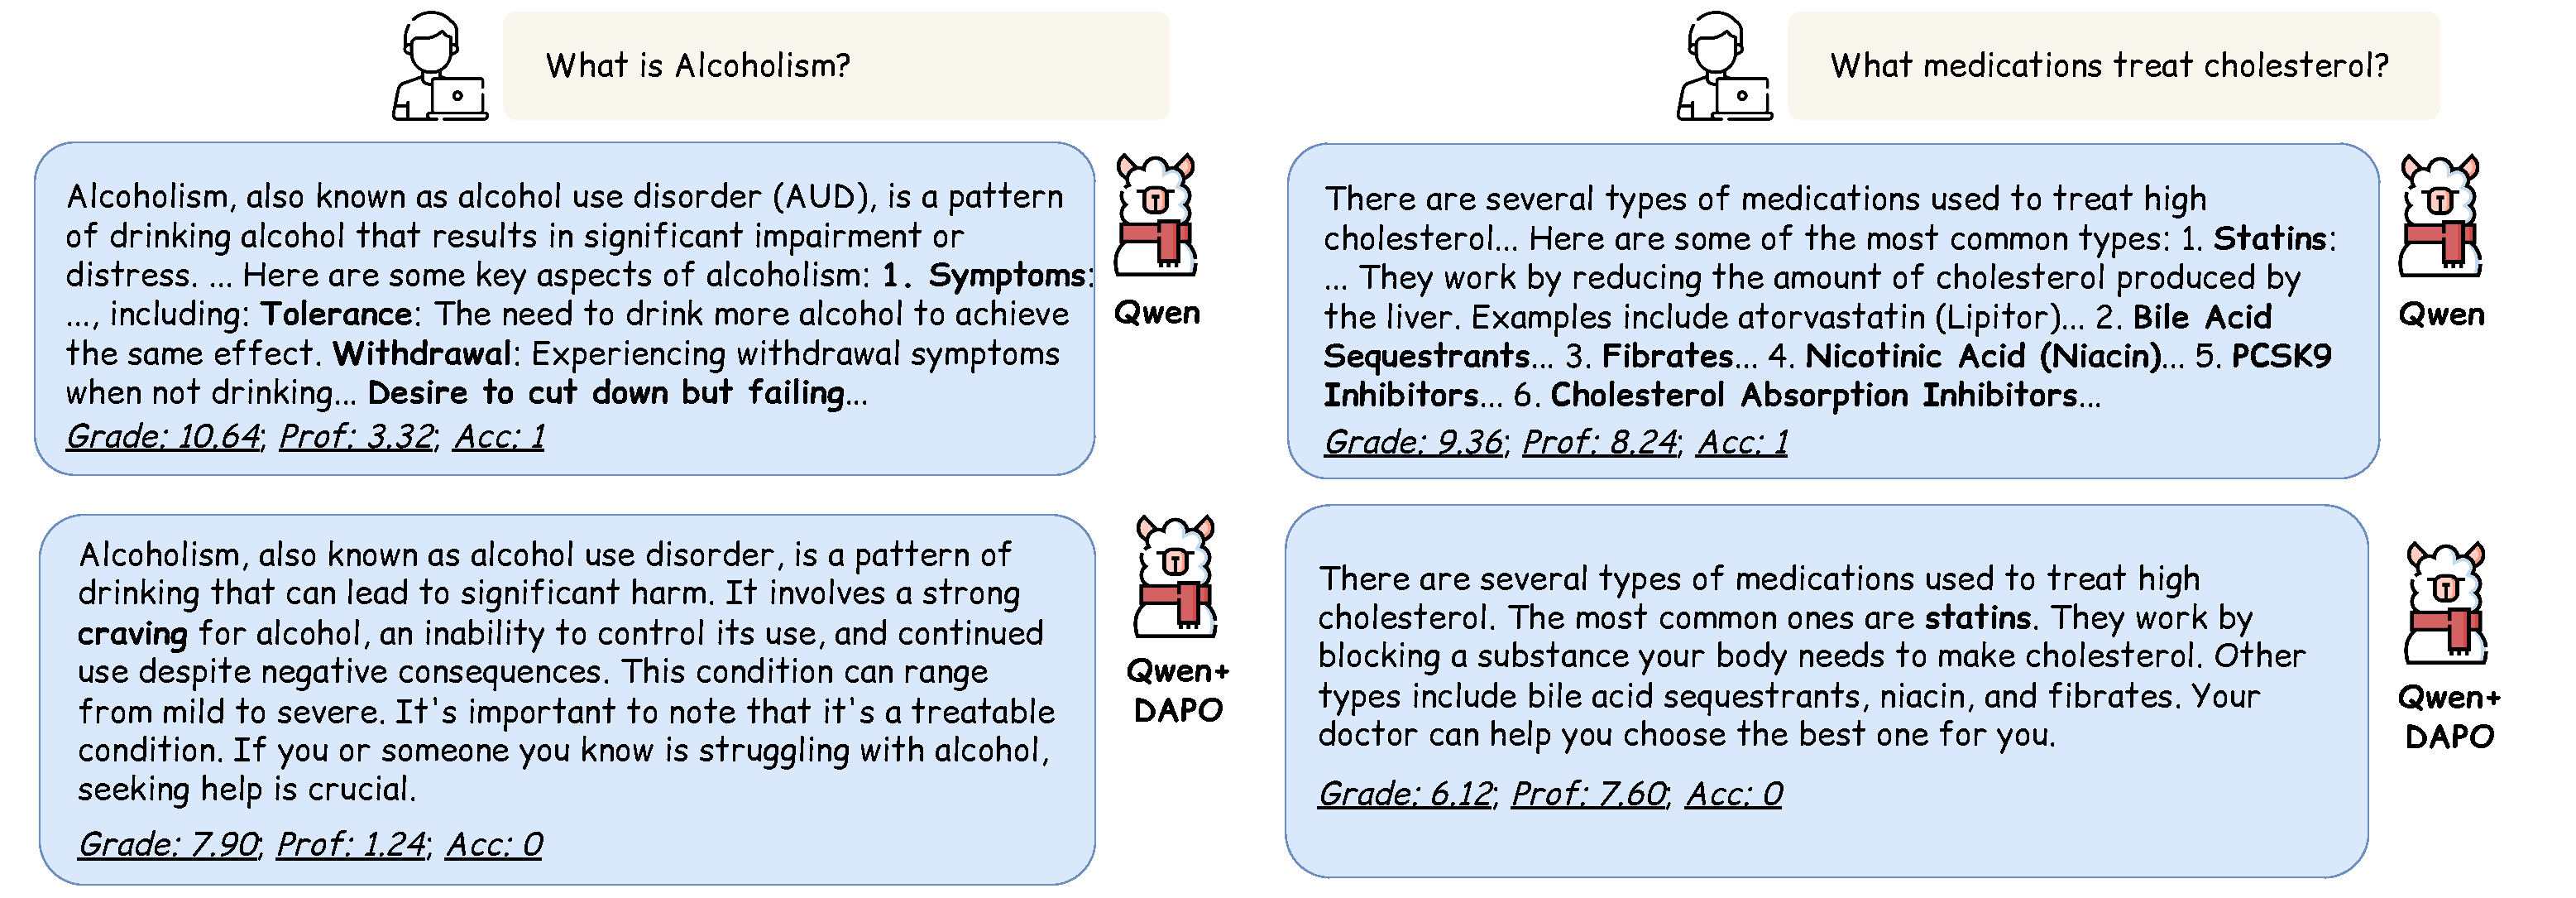
\includegraphics[width=1.\linewidth]{figs/fail_case_studyv2.pdf}
    \caption{Examples of improved readability but reduced accuracy.}
    \label{fig:fail_case}
\end{figure}

To illustrate this trade-off, Figure~\ref{fig:fail_case} presented two cases where DAPO yielded simpler text but missed key facts relative to the base model.
In particular, the DAPO model tended to over-simplify, compressing lists and collapsing categories, so that only a salient term was retained (e.g., \emph{craving} for alcohol use disorder; \emph{statins} for cholesterol drugs) while other classes (e.g., bile-acid sequestrants, fibrates, niacin, PCSK9 inhibitors) were merged into a single undifferentiated sentence, leading to information loss.

\section{Discussion}\label{sec:discussion}

In this study, we examined a critical yet underexplored factor in developing effective patient education agents, i.e., the readability of LLM-generated responses, through \bench, a benchmark of expert-grounded patient education QA pairs.
\bench comprises 533 QA pairs curated from 27 authoritative online resources and reviewed by professionals in nursing, public health, and clinical communication, together with a large-scale collection of 36,060 public health questions used to explore strategies for improving readability.
Unlike prior healthcare benchmarks, which primarily assess the factual or reasoning accuracy of LLMs against professional examinations or specialized clinical tasks, \bench is designed around the needs of lay users and couples three readability metrics (Flesch--Kincaid grade, professional-language proportion, and Yngve depth) with an informativeness metric that measures how much of an expert-grounded reference answer a response conveys.

Our evaluation of 19 LLMs revealed a consistent and important limitation of current systems: they struggled both to follow targeted readability instructions and to recognize the reading level required by a question or exhibited by a response.
Models generally adjusted readability in the right direction but remained poorly calibrated in absolute terms, systematically undershooting higher target grade levels, and their ability to detect high-difficulty questions and high-grade text was uniformly weak.
Together, these observations pointed to a gap between raw reasoning ability and effective communication: stronger reasoning does not automatically translate into responses that lay users can understand.

We further benchmarked several existing readability-enhancement strategies spanning test-time control (standard prompting, chain-of-thought, and readability-guided lookahead decoding) and reinforcement-learning fine-tuning (GRPO and DAPO).
We found that test-time controls traded off unevenly across readability axes, e.g., prompting lowered word-level grade and jargon but increased syntactic complexity and eroded informativeness, whereas reinforcement learning was the only family of methods that improved word choice, syntax, and faithfulness jointly.
Among them, DAPO yielded the largest readability gains, reducing the grade level by 41.4\% and the professional-language score by 73.3\% on average.
However, these gains can come at the expense of informativeness, particularly for \textit{Suggestion} and \textit{Fact} questions, as models over-simplified by compressing lists and collapsing categories. This exposed a fundamental readability–informativeness trade-off that must be navigated when building accessible healthcare agents.

A further observation concerns the evaluation of readability itself.
In a blind expert evaluation, domain experts favored responses from a model that the static metrics ranked lower, indicating that automated readability metrics, while useful and scalable, may diverge from human perception of clarity and usefulness.
This motivates future work on readability measures and reward signals that better align with expert and patient judgments, as well as methods that preserve essential clinical content while simplifying language, for example by substituting jargon with plain-language equivalents rather than discarding it.

In conclusion, building user-centered public health agents requires explicitly optimizing for readability without sacrificing informativeness, an objective that current LLMs and existing enhancement strategies only partially achieve.
By providing an expert-grounded benchmark, complementary readability and informativeness metrics, and a large-scale training corpus, \bench offers a foundation for studying and improving this trade-off, and we hope it will guide the development of more accessible and trustworthy LLM-powered healthcare agents.

\textbf{Limitations.}
We focused on English content and lay users in the U.S. healthcare context. As such, the generalizability of our findings to other languages, cultures, or health systems remains limited. In addition, the readability metrics adopted here, although standard and complementary, are imperfect proxies for human comprehension, as highlighted by our expert evaluation.

\section{Methods}\label{sec:methods}

In this section, we detail the construction of \repqa, the evaluation metrics, the readability-enhancement strategies we benchmarked, the study design behind our three research questions, and the experimental setup.

\subsection{Dataset construction}\label{sec:dataset_curation}

\paragraph{Expert-grounded patient education QA.}
We collected a diverse set of publicly available healthcare-related QA pairs from 27 authoritative online resources covering a broad range of public health topics, including general health, cardiovascular disease, cholesterol, diabetes, HIV, diet, exercise, alcohol, smoking, sleep, mental health, sexual health, and health equity.
Sources were selected for their accessibility to lay audiences and their coverage of frequently asked questions by the general public.
For the evaluation dataset, domain experts further manually filtered out QA pairs containing overly technical content, following national, authoritative research and clinical guidelines~\citep{doody2016nursing,chiang2016guidance,corry2013developing}.
Questions are phrased in plain language and do not include user profiles.

The resulting evaluation dataset includes 533 QA pairs spanning four categories, i.e., \textit{Suggestion}, \textit{Fact}, \textit{Definition}, and \textit{Rationale}, as summarized in Table~\ref{tab:dataset_category}:
\begin{itemize}[leftmargin=*]
\item \textit{Suggestion}: Questions seeking advice. These responses must be highly readable to ensure that users can easily follow recommendations without ambiguity.

\item \textit{Fact}: Questions requesting objective, verifiable information. Presenting facts in lay-accessible language is essential for avoiding misinterpretation.

\item \textit{Definition}: Questions asking for explanations of medical terms or conditions. Definitions require high readability, as they often introduce unfamiliar terminology.

\item \textit{Rationale}: Questions seeking justifications behind medical guidance. These responses must balance clarity with accuracy in plain language to build user understanding.
\end{itemize}

\paragraph{Large-scale healthcare questions.}
In addition to the evaluation QA pairs, we curated a large-scale collection consisting of 36,060 public health questions.
These queries span an extensive range of public health topics, including sleep, exercise, smoking, weight, diet, HIV care, mental health, cardiovascular disease, diabetes, cholesterol, and SOGI, drawn from 52 publicly available resources.
The data sources were manually selected by nursing and public health professionals, following the same guidelines used in curating the evaluation dataset.
Summary statistics and representative examples for each category are presented in Table~\ref{tab:training_dataset}. For each question, the reference answer was generated by GPT-4o-mini using supporting materials as context. During post-training, this context was not used to train the model’s parametric knowledge. The datasets were subsequently reviewed by domain experts to ensure quality.


\begin{table*}[t]
    \centering
    \caption{Examples and distribution of question categories in the collected training datasets. A single question can be categorized into multiple categories.}
    \resizebox{\textwidth}{!}{
    \begin{tabular}{clc}
    \toprule
    Category & Example & Proportion \\
    \midrule
    \midrule
    Sleep & How does sleep apnea during pregnancy potentially affect newborns? & 8.1\% \\
    Exercise & What are some effective strategies for improving family health through physical activities? & 6.3\% \\
    Smoking & What are some effective strategies individuals can use to quit smoking and support a smoke-free lifestyle? & 4.5\% \\
    Weight & How is body mass index (BMI) calculated, and what factors can affect its accuracy? & 7.2\% \\
    Diet & How can someone maintain a healthy diet while dining out? & 10.3\% \\
    HIV Care & How can gay men effectively manage their risk of HIV? & 14.4\% \\
    Mental Health & How can parents support the mental health of their children? & 12.6\% \\
    Cardiovascular & What is the primary difference between cardiac arrest and a heart attack? & 18.7\% \\
    Diabetes & How do BMI categories relate to the risk of type 2 diabetes across different age groups? & 5.2\% \\
    Cholesterol & What is the significance of LDL and HDL cholesterol in relation to heart health? & 5.1\% \\
    SOGI & How can schools and communities support LGBTQI+ youth to create a safer environment? & 12.4\% \\
    Others & What are the potential benefits of utilizing specialized healthcare models in patient treatment? & 33.7\% \\
    \bottomrule
    \end{tabular}
    }
    \label{tab:training_dataset}
\end{table*}

\subsection{Evaluation metrics}\label{subsec:metrics}

We evaluated responses with a suite of four complementary metrics: three readability metrics, i.e., the Flesch--Kincaid grade level (FK), the professional-language proportion (PL), and the Yngve depth (YD), and one informativeness metric, the informative cosine (IC) between a response and its reference answer. The three readability metrics capture word difficulty, domain-specific jargon, and syntactic complexity, respectively, while IC measures how much of the reference answer's content the response conveys.

\paragraph{Flesch-Kincaid grade level (FK).}
We used the Flesch-Kincaid grade level~\citep{kincaid1975derivation} as one of our readability metrics, an established standard for assessing reading difficulty that ranges from kindergarten to post-graduate levels.
The calculation is based on the average number of syllables in a word and the average number of words in a sentence:
\begin{equation}
\label{equ:grade}
    \pi = 0.39\left(\frac{\text{\#Words}}{\text{\#Sentences}}\right) + 11.8\left(\frac{\text{\#Syllables}}{\text{\#Words}}\right) - 15.59
\end{equation}
The intuition is that sentences with many words, or words with numerous syllables, are generally more difficult to read, corresponding to a higher Flesch-Kincaid grade level.
The range of grade levels can be categorized into different school levels, e.g., 6--9 corresponds to the middle school level.

\paragraph{Professional language (PL).}
During communication between the agent and lay users without a medical background, the frequency of professional terms can significantly affect the user's reading experience.
In light of this, we incorporated the proportion of health-related professional terms in the text as one of our readability metrics:
\begin{equation}
\label{equ:prof}
    \rho = 100\% \cdot \frac{\text{Total Professional Terms}}{\text{Total Words}}
\end{equation}
We compiled a list of professional terms from the Harvard Medical Dictionary\footnote{\url{https://www.health.harvard.edu/a-through-c}}, resulting in a vocabulary of 2,058 terms.
This metric complements the Flesch-Kincaid grade level by incorporating domain-specific terminology, which may affect comprehension for lay audiences but is not captured by traditional readability formulas. A lower PL indicates fewer jargon terms and is preferable for lay readers.

\paragraph{Yngve depth (YD).}
The Flesch--Kincaid grade and professional language capture word- and term-level difficulty, but not the syntactic complexity of a response, which also affects how easily lay users can follow it.
To capture this dimension, we adopted the Yngve depth~\citep{yngve1960model}, a measure of syntactic complexity derived from the constituency parse of a sentence.
Concretely, we parse each sentence and, for every word, accumulate the left-branching load along its path from the root, i.e., the number of as-yet-unexpanded sibling constituents to its right at each step; YD is the mean of these per-word depths, averaged over sentences.
Deeper, more nested, or more heavily left-branching structures yield a higher Yngve depth, so a lower YD corresponds to simpler, easier-to-follow syntax.

\paragraph{Informative cosine (IC).}
Readability metrics alone do not penalize a response that is easy to read but omits the essential content, so we additionally measured how much of the reference answer's information a response conveys.
Each evaluation question is paired with an expert-grounded reference answer.
We embedded both the model response and the reference answer with a sentence encoder (\texttt{all-MiniLM-L6-v2}~\citep{wang2020minilm}) and computed the cosine similarity between the two embeddings:
\begin{equation}
\label{equ:ic}
    \text{IC} = \frac{\mathbf{e}_{\text{resp}} \cdot \mathbf{e}_{\text{ref}}}{\lVert \mathbf{e}_{\text{resp}} \rVert \, \lVert \mathbf{e}_{\text{ref}} \rVert}
\end{equation}
A higher IC indicates that the response is more semantically aligned with the reference answer, and thus more informative. An ideal healthcare agent should produce responses that are both easy to understand (low FK toward the target, low PL, low YD) and informative (high IC).

\subsection{Readability-enhancement strategies}\label{sec:strategies}

Beyond evaluating off-the-shelf models, we benchmarked five strategies for steering responses toward the target reading level, grouped into training-free controls and reinforcement-learning fine-tuning. The first three are applied to a frozen base model and require no parameter updates:
\begin{itemize}[leftmargin=*]
\item \textbf{Prompt}: instruction-based control, in which the base model is prompted to answer in simple, plain language at roughly a 5th-grade level, using short sentences and minimal medical jargon~\citep{ribeiro-etal-2023-generating,malik2024tarzan}.
\item \textbf{CoT}: chain-of-thought prompting~\citep{wei2022chain}, which instructs the model to reason step by step before producing its final answer; only the final answer is scored.
\item \textbf{Lookahead}: readability-guided lookahead decoding~\citep{ribeiro-etal-2023-generating}. At each decoding step, the top candidate tokens are each extended by a short greedy rollout, the rollouts are scored by how close their Flesch--Kincaid grade is to the target, and the next-token log-probabilities are biased toward the candidate whose readability is closest to the target.
\end{itemize}
The remaining two fine-tune the base model with readability as a verifiable reward (Eq.~\ref{equ:reward}): \textbf{GRPO}~\citep{shao2024deepseekmath} and \textbf{DAPO}~\citep{yu2025dapo}, where DAPO improves training stability over GRPO via decoupled clipping and dynamic sampling. We applied these strategies to three open-source base models (LLaMA3.1-8B, Qwen3-8B, and Qwen3-4B).

\subsection{Study design}\label{sec:questions}

Using \repqa, we studied LLMs' ability to adapt, assess, and optimize readability. We posed three research questions.

\paragraph{RQ1: Can LLMs generate responses at a specified reading level?}
People with different educational backgrounds have varying health literacy.
Therefore, healthcare agents should adapt the readability of their answers to a requested level (e.g., 5th grade or middle school).
We examined whether LLMs follow explicit readability instructions without sacrificing informativeness.
We compared each response's Flesch–Kincaid grade to the requested level and assessed informativeness via the informative cosine (IC).
In addition, we evaluated LLMs' readability-understanding capability: LLMs were asked to predict the reading level of given responses, and we quantified their accuracy against the Flesch–Kincaid grade.

\paragraph{RQ2: Can LLMs determine what readability is needed for a given question?}
Oversimplifying medical content omits qualifiers and loses information, while overly technical language reduces accessibility. Thus, selecting an appropriate reading level for each question is critical.
We investigated whether an LLM can infer the target level from the question alone (without user metadata).
Concretely, we extended each question in \repqa into three variants that differ in required medical knowledge, and evaluated the accuracy of the models' predictions.

\paragraph{RQ3: Can readability serve as a reward signal?}
Reinforcement learning has shown promise for steering LLMs toward preferred behaviors. We studied whether readability can act as a useful reward to drive responses toward a requested level without sacrificing content quality.
Specifically, the reward combines the evaluation metrics, i.e., the three readability metrics and the informativeness metric, so that the policy is rewarded for being both easy to read and faithful to the reference answer:
\begin{equation}
\label{equ:reward}
r = -\Big(\alpha\,|\pi - 6| + \beta\,\rho + \gamma\,\max(0,\, \text{YD} - \delta_0) + \eta\,\max(0,\, L - L_{\max})\Big) + \mu\,(\text{IC} - 1),
\end{equation}
where $\pi$ is the Flesch--Kincaid grade (Eq.~\ref{equ:grade}), $\rho$ the professional-language proportion (Eq.~\ref{equ:prof}), $\text{YD}$ the Yngve depth, and $\text{IC}$ the informative cosine (Eq.~\ref{equ:ic}); $\alpha$, $\beta$, $\gamma$, $\eta$, and $\mu$ are weights that balance the components.
A Flesch--Kincaid grade closer to $6$ (the middle-school reading level), a lower professional-language proportion, a lower Yngve depth above the baseline $\delta_0$, and a higher informative cosine (closer to the reference) all increase the reward, while an auxiliary penalty discourages responses longer than a token budget $L_{\max}$.
The informativeness term subsumes the trivial-answer penalty used in prior formulations: a content-free response has low similarity to the reference and is therefore penalized automatically.
We optimized this reward with the two reinforcement-learning algorithms described in Section~\ref{sec:strategies} (GRPO and DAPO), and compared them against the training-free controls (Prompt, CoT, and Lookahead).

\subsection{Experimental setup}\label{sec:exp_setup}

We presented an evaluation of 19 LLMs, including 5 proprietary models and 14 open-source models.
For proprietary models, we considered the GPT-5 series (GPT-5.1, GPT-5.4, and GPT-5.5)~\citep{openai2025gpt5} and GPT-4.1 (including GPT-4.1-mini)~\citep{openai2024gpt4technicalreport,openai2024gpt4ocard}.
For open-source models, we used the LLaMA~3.1 series~\citep{grattafiori2024llama3herdmodels}, the Qwen-2.5 and Qwen-3 series~\citep{qwen2.5}, Phi-4~\citep{abdin2024phi4technicalreport}, Mistral~\citep{jiang2024mixtralexperts}, BioMistral~\citep{labrak2024biomistralcollectionopensourcepretrained}, InternLM3~\citep{cai2024internlm2}, Gemma-3~\citep{gemmateam2025gemma3}, and Yi-1.5~\citep{ai2025yiopenfoundationmodels}.
We used their instruction-tuned versions by default.

\section{Conclusion}

\repqa{} showed that models often missed requested reading levels and struggled to select an appropriate level for a question. Readability-oriented post-training improved measured readability but could reduce informativeness, exposing a trade-off in adapting answers to lay readers. These findings motivate attention to how information is represented at the interface between people and machines. The following chapters turn from language-based communication to learning from brain activity. Before neural signals can support richer interfaces, their informative structure must be identified. Chapter~\ref{chapter:hybrid} addresses this problem through \hybrid{}, which learns higher-order relationships among brain regions for cognitive prediction.
